\chapter{ГЕНЕРАЦИЯ ДОПОЛНИТЕЛЬНОЙ ИНФОРМАЦИИ}
\label{chap:SIG}

\section{Вводные замечания}
\label{chap:SIG:Intro}

Настоящий раздел посвящен задаче генерации дополнительной информации декодера в распределенных видеокодеках. В начале приводится обзор типовых подходов к решению данной задачи и выделяется ключевая операция, связанная с оценкой движения между кадрами видеопоследовательности. Далее дается краткое описание метода оценки движения, используемого при генерации дополнительной информации в базовой модели распределенного кодирования на базе проекта DISCOVER, указываются его основные особенности и потенциальные недостатки. В настоящем разделе данный алгоритм считается базовым для последующего анализа и улучшений. Далее вводится в рассмотрение понятие <<истинного движения>> как векторного поля, отражающего реальное смещение объектов между парой кадров видеопоследовательности. Данное понятие затем формализуется с использованием оптимизационной задачи и приводится описание нового эвристического алгоритма оценки истинного движения, выполняющего поиск локального минимума введенной оптимизационной задачи. Объяснение сходимости алгоритма к некоторому локальному минимуму дается на качественном уровне. Вопросы, связанные с оценкой эффективности данного алгоритма, рассматриваются в разделе~\ref{chap:ExpResults}. Основные результаты данного раздела опубликованы в работах~\cite{VeselovMonograph},~\cite{6958822},~\cite{VeselovIus}.

\section{Обзор методов генерации дополнительной информации}
\label{chap:SIG:Review}

Как было показано в подразделе~\ref{chap:DVC:Arhcs:Stan}, процедура генерации дополнительной информации выполняется декодером для формирования вспомогательных данных, которые интерпретируются как выход одного из зависимых источников в схеме распределенного кодирования. При обработке видеоданных ключевым методом процесса генерации дополнительной информации является выполнение на стороне декодера предсказания промежуточного кадра по ранее декодированным кадрам видеопоследовательности~\cite{VeselovMonograph}. В зависимости от того, какой подход лежит в основе процедуры предсказания, выделяют два класса методов генерации дополнительной информации:
\begin{itemize}
    \item подходы, основанные на временной интерполяции~\cite{Huang2008};
    \item подходы, основанные на временной экстраполяции~\cite{Tome2009}.
\end{itemize}
В схемах, основанных на экстраполяции, для формирования дополнительной информации используются только кадры видеопоследовательности, предшествующие во времени предсказываемому кадру. Существенным преимуществом такого подхода является то, что не увеличивается задержка декодирования, т.~к. поток кадров декодируется в том же порядке, в котором он поступает на вход кодера. Однако, в силу того что при экстраполяции не доступна информация о реальном движении объектов на будущих кадрах, данный метод может в общем приводить к большему числу ошибок по сравнению с методами, основанными на интерполяции.

В подходах, основанных на интерполяции, для предсказания промежуточного кадра используются как кадры из прошлого, так и кадры из будущего. Таким образом, на декодере необходимо сначала восстановить так называемые опорные кадры, а затем по ним осуществить интерполяцию, что позволяет выполнять предсказание точнее по сравнению с экстраполяцией, но приводит к увеличению задержки декодирования. Однако, т.~к. данный недостаток, как правило, не является критичным для типовых сценариев применения распределенного кодирования видеоданных, именно подходы использующие интерполяцию кадров получили наибольшее распространение.

Обобщенная схема типового метода межкадрового предсказания, основанного на временной интерполяции кадров, приведена на рисунок~\ref{fig:GenericInterpolation}. Она включает два основных блока:
\begin{itemize}
\item блок оценки движения (Motion Estimation, ME), используется для оценки изменений между соседними кадрами;
\item блок компенсации движения, используется для формирования нового кадра с использованием информации от предыдущего блока.
\end{itemize}
\begin{figure}[htbp]
    \begin{center}
        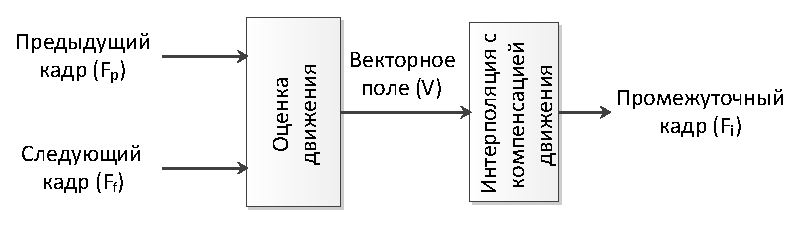
\includegraphics[width=0.9\textwidth]{Chapter2/GenericInterpolation}
        \caption{Обобщенная схема типового алгоритма временной интерполяции}
        \label{fig:GenericInterpolation}
    \end{center}
\end{figure}
Перед тем, как переходить к описанию особенностей процедуры предсказания кадров с использованием временной интерполяции введем ряд необходимых определений.
\begin{definition}
    Будем называть \emph{вектором движения} двумерный вектор, показывающий изменение координат пикселя между кадрами.
\end{definition}
\begin{definition}
    \emph{Векторное поле} -- матрица, содержащая векторы движения всех пикселей кадра, для которого выполняется процедура оценки движения.
\end{definition}
В схеме предсказания кадров назначение блока оценки движения заключается в поиске такого векторного поля, которое отражает перемещение объектов на оригинальных кадрах видеопоследовательности. Эта задача известна как поиск \emph{истинного движения} (True Motion Estimation)~\cite{Chen1998}.
\begin{definition}
    \emph Векторное поле, соответствующее истинному движению, будем называть \emph{истинным векторным полем}.
\end{definition}
Истинное векторное поле используется в блоке компенсации движения для интерполяции объектов на промежуточных кадрах в тех координатах, в которые объекты должны сместиться в соответствии с траекторией их движения в видеопоследовательности.

Можно выделить две основные задачи, возникающие при временной интерполяции кадров:
\begin{enumerate}
\item поиск истинного движения~\cite{Haan1993};
\item обработка регионов на интерполированном кадре, не имеющих вектора движения или имеющих более одного вектора движения~\cite{Bartels2009}.
\end{enumerate}
Следует отметить, что задача поиска истинного движения отличается от задачи оценки движения, возникающей при сжатии видеопоследовательностей. В связи с этим для формализации понятия истинного движения, как правило, используется ряд допущений о типовом векторном поле, отражающем специфику перемещений объектов на кадрах. Одним из наиболее распространенных допущений является допущение о гладкости векторного поля, заключающееся в том, что векторы движения, соответствующие пространственно близким регионам, должны быть похожи. При этом под похожестью векторов понимается как похожесть амплитуды, так и направления. Как правило, для расчета гладкого векторного поля используются схемы, основанные на предсказании векторов движения, в которых поиск вектора для нового региона осуществляется с учетом векторов, сформированных ранее для соседних регионов. Процедура предсказания может осуществляться как в пространственной области, так и во временной. Однако, допущение о гладкости векторного поля, как правило, является неверным для регионов, содержащих границы объектов. При поиске истинного движения для таких регионов используется предсказание с учетом векторов, полученных по обе стороны границы объекта. Предсказанные направления затем используются для инициализации векторов, соответствующих региону, содержащему границу. Подобный подход используется в одном из первых алгоритмов поиска истинного движения~--~\emph{трехмерном рекурсивном поиске} (3D Recursive Search~--~3DRS)~\cite{Haan1993}.

Вторая задача временной интерполяции связана с назначением векторов движения областям на интерполированном кадре. Существует два основных подхода к решению этой задачи:
\begin{enumerate}
\item однонаправленная оценка/компенсация движения~\cite{Haan1993};
\item двунаправленная (билатеральная) оценка/компенсация движения~\cite{Choi2000}.
\end{enumerate}
В соответствии с однонаправленным подходом один из смежных базовых кадров разбивается на непересекающиеся блоки, и для каждого блока ищется наиболее похожий блок в другом кадре. Вектор движения определяется как расстояние между координатами этих блоков на кадрах. Координаты блока на промежуточном кадре находятся посередине между координатами блоков на базовых кадрах. Интерполяция осуществляется усреднением пикселей, находящихся на совпадающих позициях в блоках и помещением нового <<усредненного>> блока в соответствующую позицию на промежуточном кадре. У такого подхода есть существенный недостаток, поскольку в промежуточном кадре возможно появление регионов, для которых интерполяция с использованием найденных вектором будет неоднозначна:
\begin{itemize}
\item области, не ассоциированные ни с одним из найденных векторов (так называемые <<дыры>>);
\item регионы, которые ассоциированы с несколькими найденными векторами (так называемые <<наложения>>).
\end{itemize}
Двунаправленный подход позволяет избежать этих проблем. Основным допущением билатерального подхода является допущение о равномерности и прямолинейности движения объектов. В таком случае на блоки разбивается не один из опорных кадров, а промежуточный кадр. Для каждой фиксированной позиции блока на промежуточном кадре осуществляется поиск похожих блоков на оригинальных кадрах, при котором векторы смещения коллинеарны, разнонаправлены и откладываются относительно блока в промежуточном кадре. Этот подход не решает проблемы, возникающие из-за появления/исчезновения/наложения объектов на кадрах, но, в отличие от однонаправленного поиска, предоставляет завершенную процедуру обработки регионов возле этих объектов.

Следует отметить, что процедура временной интерполяции является только частью генерации дополнительной информации. Полученная аппроксимация промежуточного кадра далее, по аналогии с кодером, подвергается спектральному преобразованию и квантованию. Квантованные коэффициенты затем разбиваются на битовые плоскости, и именно битовые плоскости являются дополнительной информацией. Тем не менее, далее в данном разделе рассматривается только задача межкадрового предсказания на основе временной интерполяции, т.~к. основная причина наличия ошибок в дополнительной информации связана именно с ошибками аппроксимации.

\section{Аппроксимация промежуточных кадров в модели DISCOVER}
\label{chap:SIG:ReferenceAlgo}

\subsection{Основные определения и обозначения}
\label{chap:SIG:ReferenceAlgo:Notation}

При описании алгоритма оценки движения будем рассматривать пару соседних кадров оригинальной видеопоследовательности $\mathbf{F}_p$ и $\mathbf{F}_f$, между которыми необходимо построить векторное поле $\mathbf{V}$, описывающее смещение объектов между этими кадрами. Кадры $\mathbf{F}_p$ и $\mathbf{F}_f$ будем называть опорными или базовыми кадрами. Матрица векторов движения $\mathbf{V}$ (векторное поле) используется для интерполяции нового кадра $\mathbf{F}_i$, расположенного во времени между базовыми кадрами. Кадр $\mathbf{F}_i$ будем называть интерполированным или промежуточным кадром. Здесь и далее будем считать, что обрабатываемые кадры являются многокомпонентными (или цветными) изображениями, представленными одной яркостной компонентой Y и двумя хроматическими компонентами Cb и Cr. Однако следует отметить, что описанные далее алгоритмы легко обобщаются на изображения с произвольным числом компонент.

\begin{figure}[th]
\begin{center}
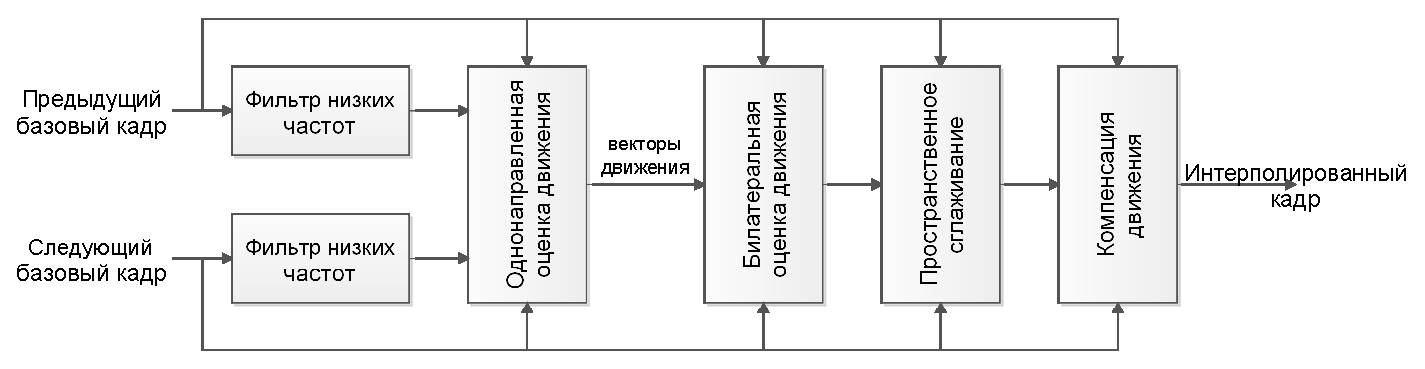
\includegraphics[width=0.9\textwidth]{Chapter2/DiscoverSIG}
\end{center}
\caption{Схема алгоритма межкадрового предсказания в модели DISCOVER}
\label{fig:ch2:DiscoverSIG}
\end{figure}

Перед тем, как приводить подробное описание процедуры аппроксимации, рассмотрим её основные этапы и их назначение. В модели DISCOVER оценка движения реализуется за два шага (рисунок~\ref{fig:ch2:DiscoverSIG})~\cite{Ascenso2006},~\cite{Ascenso2005}. На первом шаге выполняется однонаправленная оценка движения, на втором – билатеральная. Перед первым шагом оба базовых кадра подвергаются низкочастотной фильтрации для уменьшения шумов. Считается что такого рода предобработка способствует повышению точности оценки движения. После однонаправленной оценки выполняется уточняющая билатеральная оценка с меньшим радиусом поиска.
На всех шагах используется блоковая оценка движения, т.е. один из кадров разбивается на непересекающиеся квадратные блоки пикселей. Для каждого такого блока определяется \emph{вектор движения} $\mathbf{v}=(v_y,v_x)^T$, соответствующий изменению координат $y$ и $x$ этого блока между ключевыми кадрами. В качестве критерия, по которому оценивается изменение местоположения блока, в DISCOVER используется среднеквадратичное искажение (MSE, Mean Squared Error).

Введем необходимые обозначения. Для упрощения изложения будем полагать, что выполняются следующие соотношения:
\begin{equation*}
\frac{w}{b}, \frac{h}{b} \in \mathbb{N},
\end{equation*}
где $w$ и $h$~--~ширина и высота кадров соответственно; $b$~--~размер блока, для которого выполняется оценка движения.

Назовем множество координат пикселей на кадре сеткой пикселей. Формально сетку пикселей можно определить как
\begin{equation*}
\mathcal{P} = \lbrace \mathbf{p}=(y,x)^T \vert y \in \mathcal{Y}, x \in \mathcal{X} \rbrace,
\end{equation*}
где $\mathcal{X}=\lbrace 1,2,...,w \rbrace $, $\mathcal{Y}= \lbrace 1,2,...,h \rbrace $. В общем случае значение пикселя в координате $\mathbf{p}=(y,x)^T$ на кадре $\mathbf{F}$ задается как триплет $\mathbf{F}(\mathbf{p})=(\mathbf{Y}(\mathbf{p}),\mathbf{Cb}(\mathbf{p}),\mathbf{Cr}(\mathbf{p}))$, однако, т.~к. в модели DISCOVER обрабатываются только последовательности с кадрами в градациях серого, будем рассматривать только обработку яркостной компоненты, т.~е. будем считать, что  $\mathbf{F}(\mathbf{p})=\mathbf{Y}(\mathbf{p})$.
По аналогии с сеткой пикселей определим сетку блоков, как множество координат блоков (координат левого верхнего пикселя в блоке) на кадре:
\begin{equation*}
\mathcal{G} = \lbrace \mathbf{g}_{i,j}=(i,j)^T \vert i \in \mathcal{I}, j \in \mathcal{J} \rbrace,
\end{equation*}
где $\mathcal{I}=\lbrace 1,2,...,\frac{h}{b}\rbrace$, $\mathcal{J}=\lbrace 1,2,...,\frac{w}{b}\rbrace$~--~высота и ширина сетки блоков соответственно. 

Множество координат пикселей, находящихся в блоке с индексом $(i, j)^T$ определим как
\begin{equation*}
\mathcal{B}_{i,j} = \lbrace (y,x)^T \in \mathcal{P} \vert y \in \mathcal{Y}_i, x \in \mathcal{X}_j \rbrace,
\end{equation*}
где $\mathcal{Y}_i=\lbrace (i-1)b+1,..., ib \rbrace$; $\mathcal{X}_j=\lbrace (j-1)b+1,..., j b\rbrace$.

Приведем описание алгоритма межкадрового предсказания в модели DISCOVER с учетом введенных обозначений.

\subsection{Однонаправленная оценка движения}

Поиск векторов движения осуществляется как оценка смещения в последующем ключевом кадре $\mathbf{F}_f$ относительно предыдущего $\mathbf{F}_p$. Для каждого блока на предыдущем ключевом кадре ищется вектор движения с минимальной ошибкой сопоставления блоков:

\begin{equation*}
\mathbf{v}_{i,j}^{(u)} = \arg\min_{\mathbf{v} \in \mathcal{V}_{s}^{(u)}} \frac{1}{b^2} \sum\limits_{\mathbf{p} \in \mathcal{B}_{i,j}} (\mathbf{F}_p(\mathbf{p}) - \mathbf{F}_f(\mathbf{p}+\mathbf{v}))^2,
\end{equation*}
где $\mathcal{V}_{s}^{(u)}=\{ (-r,-r)^T, (-r+\delta,-r)^T, (-r,-r+\delta)^T, \cdots, (r,r)^T \}$~--~множество возможных векторов движения; $r$ - радиус поиска, определяющий максимальную длину вектора, $\delta$ - расстояние между векторами.

Таким образом, на первом шаге для каждого блока на предыдущем кадре ищется с помощью перебора векторов в некотором радиусе оптимальный вектор движения, соответствующий минимальному среднему квадрату ошибки сопоставления блоков. Данный вектор соответствует смещению всех пикселей в блоке между кадрами. Координаты пикселя на интерполированном кадре $\mathbf{F}_i$ рассчитываются по правилу:

\begin{equation*}
\mathbf{p}_i = \mathrm{round}(\mathbf{p}_p + \alpha\mathbf{v}),
\end{equation*}
где $\mathbf{p}_i=(y,x)_i^T$ и $\mathbf{p}_p=(y,x)_p^T$~--~координаты пикселей в интерполированном и предыдущем ключевом кадрах соответственно, $\alpha=\frac{d_p}{d}$, $d$~--~расстояние (количество кадров) между ключевыми кадрами, $d_p$~--~расстояние между предыдущим опорным кадром и интерполированным кадром. Здесь и далее для упрощения обозначений будем рассматривать случай, когда $\alpha=\frac{1}{2}$, т.~е. промежуточный кадр находится посередине между базовыми.

Результатом данного поиска является векторное поле, причем векторы движения поставлены в соответствие пикселям одного из базовых кадров, что может приводить к <<дырам>> и <<коллизиям>> на промежуточном кадре. Для устранения этих эффектов на втором шаге алгоритма выполняется дополнительная билатеральная оценка движения.

\subsection{Билатеральная оценка движения}

Первой операцией билатеральной оценки является преобразование однонаправленного векторного поля, полученного с предыдущего шага алгоритма, в билатеральное. Для этого промежуточный кадр разбивается на непересекающиеся блоки и для каждого блока осуществляется выбор билатерального вектора из множества однонаправленных векторов, пересекающих этот блок. Выбор заключается в поиске такого однонаправленного вектора, который <<покрывает>> наибольшее число позиций пикселей в соответствующим блоке на промежуточном кадре.

Таким образом, в результате данного преобразования на промежуточном кадре строится сетка непересекающихся блоков, причем каждому блоку поставлен в соответствие билатеральный вектор движения, т. е. построено начальное билатеральное векторное поле. Данное поле уточняется в процессе билатеральной оценки движения.

В процессе билатеральной оценки движения на ключевых кадрах ищутся похожие блоки относительно координат $\mathbf{p}_t$ для блоков в интерполированном, анализируя разности:
\begin{equation}
\mathbf{v}_{i,j}^{(b)} = \arg\min_{\mathbf{v} \in \mathcal{V}_{i,j}^{(b)}} \frac{1}{b^2} \sum\limits_{\mathbf{p} \in \mathcal{B}_{i,j}} (\mathbf{F}_p(\mathbf{p}-\mathbf{v}) - \mathbf{F}_f(\mathbf{p}+\mathbf{v}))^2,
\label{eq:MSEDiscover}
\end{equation}
где $\mathcal{V}_{i,j}^{(b)}=\{ \mathbf{v}_{i,j}'+(-r',-r')^T, \mathbf{v}_{i,j}'+(-r'+1,-r')^T, \mathbf{v}_{i,j}'+(-r',-r'+1)^T,\ldots, \mathbf{v}_{i,j}'+(r',r')^T \}$~--~множество возможных билатеральных векторов движения, учитывающее результат однонаправленной оценки $\mathbf{v}_{i,j}'$.

Поиск векторов движения при билатеральной оценке осуществляется в радиусе $r'$ относительно начального однонаправленного смещения, причем~$r'<r$.

После билатеральной оценки у каждой координаты пикселя на промежуточном кадре будет оцененный вектор движения, т.~е. на интерполированном кадре не будет регионов с <<коллизиями>> и <<дырами>>, которые возможны после первого шага.
 
\subsection{Сглаживание векторного поля}

Следующим шагом алгоритма является пространственное сглаживание \emph{векторного поля}. Для этого используется взвешенная медианная фильтрация. Для блока с координатой $\mathbf{g}_{i,j}$ и вектором движения $\mathbf{v}_{i,j}$ эта операция определена как:
\begin{equation}
\mathbf{v}^*_{i,j} = \arg\max_{\mathbf{v}\in \{\mathbf{v}_1,...\mathbf{v}_n\}}
\left( \sum\limits_{k=1}^{n} w_k ( \lVert\mathbf{v}_{i,j} - \mathbf{v}_k\rVert_L - \lVert\mathbf{v} - \mathbf{v}_k\rVert_L ) \right),
\end{equation}
где $\mathbf{v}^*_i$~--~результат фильтрации, $\{\mathbf{v}_1,\ldots,\mathbf{v}_n\}$~--~множество участвующих в фильтрации $\mathbf{v}_i$ векторов, в это множество входят векторы соседних блоков, а также вектор для блока на позиции $\mathbf{g}_{i,j}$, найденный для предыдущего интерполированном кадра; $w_k$~--~весовые коэффициенты, определяемые как:
\begin{equation}
w_k = \frac{\mathrm{MSE}(\mathbf{v}_{i,j},\mathbf{g}_{i,j})}{\mathrm{MSE}(\mathbf{v}_k,\mathbf{g}_{i,j})},
\end{equation}
где $\mathrm{MSE}(\mathbf{v},\mathbf{p})$~--~функция расчета среднеквадратичной ошибки~(\ref{eq:MSEDiscover}) при применении вектора $\mathbf{v}$ к блоку на позиции $\mathbf{p}$.
Полученное сглаженное билатеральное векторное поле $\mathbf{V}$ затем используется на последнем шаге алгоритма для выполнения компенсации движения и формирования интерполированного кадра.

\subsection{Интерполяция с компенсацией движения}

Перед этим шагом каждому пикселю на промежуточном кадре поставлен в соответствие билатеральный вектор движения, полученный в результате оценки движения для блока, в котором этот пиксель находится. Интерполяция с компенсацией движения заключается в усреднении интенсивностей соответствующих пикселей в базовых кадрах и помещении полученного значения в соответствующую координату пикселя на промежуточном кадре:

\begin{equation}
\mathbf{F}_i(\mathbf{p}) = \frac{1}{2} \left[ \mathbf{F}_p(\mathbf{p}-\mathbf{V}(\mathbf{p})) + \mathbf{F}_f(\mathbf{p}_i+\mathbf{V}(\mathbf{p}))\right], \forall \mathbf{p} \in \mathcal{P}.
\end{equation}

\subsection{Параметры процедуры аппроксимации кадров}

В завершении описания алгоритма укажем параметры, используемые в DISCOVER~\cite{Ascenso2005}:

\begin{itemize}
    \item сглаживание выполняется с использованием усредняющего фильтра размером $3\times3$ пикселя;
    \item размер блока на при однонаправленной оценке движения: $b=16$;
    \item радиус поиска при однонаправленной оценке движения: $r=32$;
    \item размер блока на при билатеральной оценке движения: $b=8$;
    \item расстояние между перебираемыми векторами: $\delta=2$;
    \item радиус поиска при билатеральной оценке движения: $r'=2$.
\end{itemize}

Oценка движения выполняется с полупиксельной точностью.

\subsection{Недостатки базового алгоритма}
\label{chap:SIG:ReferenceAlgo:Troubles}

Одним из существенных недостатков используемого в DISCOVER метода генерации дополнительной информации является то, что в нем используется обычная блоковая оценка движения с полным перебором всех возможных векторов движения в некотором радиусе. Учет корреляции векторов соседних блоков осуществляется только при билатеральном допоиске и взвешенной медианной фильтрации векторного поля, но никак не используется в самой процедуре оценки движения. Таким образом, данный алгоритм в явном виде не учитывает допущения об истинном движении, приведенные в подразделе~\ref{chap:SIG:Review}, и можно добиться существенного повышения качества аппроксимации, если учесть эти допущения при оценке движения.

\section{Модель истинного движения в задаче временной интерполяции кадров}
\label{chap:SIG:TrueMotionModel}

Перед тем, как приводить описание нового алгоритма поиска векторного поля, рассмотрим введенное ранее понятие истинного движения более формально. Будем считать, что истинное векторное поле может быть получено в результате оптимизации следующей функции при фиксированных кадрах $\mathbf{F}_p$ и $\mathbf{F}_f$~\cite{Rajala1992}:
\begin{equation}
\mathbf{V}^* = \arg\min\limits_{\mathbf{V} \in \mathcal{V}} \mathrm{E}(\mathbf{F}_p, \mathbf{F}_f, \mathbf{V})
\label{eq:MeModel}
\end{equation}
где $\mathcal{V}$ – пространство всех возможных векторных полей $\mathbf{V}$ и
\begin{equation}
\mathrm{E}(\mathbf{F}_p, \mathbf{F}_f, \mathbf{V}, \alpha) = \mathrm{E}_1(\mathbf{F}_p, \mathbf{F}_f, \mathbf{V}) + \alpha \mathrm{E}_2(\mathbf{V}).
\label{eq:MeModelExplained}
\end{equation}
Слагаемое $\mathrm{E}_1(\cdot,\cdot,\cdot)$ соответствует энергии разностного кадра между кадрами $\mathbf{F}_p$ и $\mathbf{F}_f$ с использованием векторного поля $\mathbf{V}$; слагаемое $\mathrm{E}_2(\cdot)$ отражает гладкость (похожесть соседних векторов) поля $\mathbf{V}$; $\alpha\geq0$~--~коэффициент регуляризации между энергией разностного кадра и гладкостью векторного поля. Следует отметить, что обычно $\mathrm{E}_2$ является обратным значением к гладкости, т.е. меньшее значение $\mathrm{E}_2$ соответствует более гладкому полю $\mathbf{V}$.

Сформулированную оптимизационную задачу можно пояснить следующим образом: алгоритм оценки движения должен найти такое гладкое векторное поле, которое минимизирует энергию разностного кадра. Коэффициент $\alpha$ служит для балансировки между гладкостью и энергией (ошибкой сопоставления блоков). В том случае, если значение $\alpha$ близко к нулю, оптимальное векторное поле будет доставлять глобальный минимум энергии разностного кадра, но векторы движения при этом могут быть хаотичны. С другой стороны, большое значение $\alpha$ приводит к тому, что оптимальное векторное поле может быть чрезмерно сглаженным и не обеспечивать хорошего совпадения базовых кадров. Промежуточные значения $\alpha$ соответствуют сбалансированному гладкому векторному полю, обеспечивающему приемлемое совпадение базовых кадров. Следует отметить, что $\alpha$ является одним из параметров данной модели. Поиск значения $\alpha$, соответствующего истинному движению является сложной задачей, т.к. в общем случае нельзя сказать, что зависимость значения целевой функции от $\alpha$ является унимодальной.

Предположим, что в пространстве $\mathcal{V}$ введено отношение соседства. Обозначим через $N(\mathbf{V})$ множество соседей $\mathbf{V}$ в $\mathcal{V}$. Говорят, что векторное поле $\mathbf{V}^*$ доставляет локальный минимум $\mathrm{E}(\cdot,\cdot,\cdot,\cdot)$ при фиксированных кадрах $\mathbf{F}_p$ и $\mathbf{F}_f$ тогда и только тогда, когда для всех $\mathbf{V} \in N(\mathbf{V})$ выполняется следующее соотношение:
\begin{equation}
E(\mathbf{F}_p, \mathbf{F}_f, \mathbf{V}^{*}) \le E(\mathbf{F}_p, \mathbf{F}_f, \mathbf{V}).
\label{eq:Minima}
\end{equation}
В том случае, если неравенство выполняется для всех $\mathbf{V} \in \mathcal{V}$, говорят, что векторное поле $\mathbf{V}$ доставляет глобальный минимум $E$.

Следует отметить, что существуют алгоритмы, которые для заданных $\alpha$ в некоторых случаях позволяют искать минимумы функции (\ref{eq:MeModel}) в явном виде~\cite{Boykov2004},~\cite{Morales2009}. Так как функция (\ref{eq:MeModel}) зависит от большого числа параметров и не является унимодальной, найденные минимумы являются, как правило, локальными. Однако следует отметить, что с помощью формулы (\ref{eq:MeModel}) описывается только модель движения, и векторные поля, соответствующие локальным и глобальным минимумам этой модели, не обязательно точно отражают истинное движение объектов на кадрах. В частности, модель не учитывает неравномерность движения на границах объектов, где векторное поле, как правило, не является гладким. Поэтому найденное для данной модели решение не гарантирует высокого визуального качества в результате интерполяции. В связи с этим более хорошие результаты с точки зрения визуального качества достигаются с использованием подоптимальных алгоритмов, рассматривающих оптимизацию (\ref{eq:MeModel}) неявно. Такие алгоритмы, как правило, с одной стороны основаны на эвристических подходах, нацеленных на повышение визуального качества интерполированных кадров, а с другой стороны, неявно косвенно минимизируют (\ref{eq:MeModel}), т.е. выдают результат, согласованный с моделью истинного движения. В связи с этим далее в данном разделе приводится описание алгоритма оценки движения, принадлежащего именно к такому классу алгоритмов.

Процедура поиска оптимального вектора движения, лежащая в основе всех методов оценки движения, также может быть реализована с использованием либо полного перебора всех возможных векторов (оптимальный поиск), либо с использованием некоторой под-оптимального алгоритма. Полный перебор оптимален в том смысле, что он гарантирует минимум ошибки $E_1$ в~\ref{eq:MeModelExplained}. В ряде работ~\cite{Sohn2007} указывается, что полный перебор плохо согласуется с поиском истинного движения, в особенности на текстурных регионах. Кроме того, процедура полного перебора всех векторов обладает высокой вычислительной сложностью. В связи с этим поиск оптимального вектора в задаче оценки истинного движения, как правило, осуществляется с использованием под-оптимальных методов, например, градиентного спуска~\cite{Liu1996}.

\section{Описание разработанного алгоритма аппроксимации промежуточных кадров с учетом истинного движения}
\label{chap:SIG:ProposedAlgo}

\subsection{Обоснование разработанного алгоритма}
\label{chap:SIG:ProposedAlgo:Foundation}

В основе разработанного алгоритма оценки движения (рисунок~\ref{fig:ch2:SuaiMCFI}) лежит многоуровневая иерархическая билатеральная процедура блоковой оценки движения с дополнительным итеративным поиском~\cite{VeselovIus},~\cite{6958822}. На каждом уровне иерархии для фиксированного размера блока выполняются три основные операции:
\begin{enumerate}
\item инициализация уровня иерархии для подготовки кадров к оценке движения;
\item начальная оценка движения, используемая для поиска предварительного векторного поля, доставляющего локальный минимум $E_1$ в~(\ref{eq:MeModelExplained});
\item итеративный дополнительный поиск, повышающий гладкость векторного поля (уменьшение $E_2$ в~(\ref{eq:MeModelExplained})).
\end{enumerate}

\begin{figure}[th]
\begin{center}
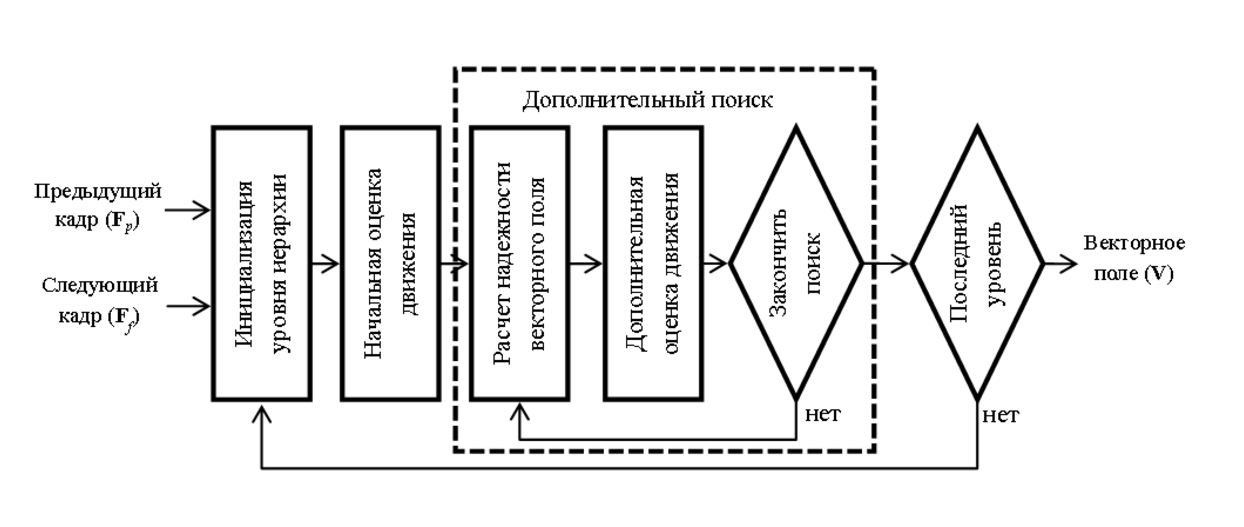
\includegraphics[width=0.9\textwidth]{Chapter2/SuaiMCFI}
\end{center}
\caption{Схема разработанного алгоритма оценки движения}
\label{fig:ch2:SuaiMCFI}
\end{figure}

На каждом уровне иерархии выполняется оценка движения для блоков фиксированного размера. Здесь и далее будем называть процесс обработки одного уровня стадией. Выходом стадии является векторное поле $\mathbf{V}^*$, доставляющее локальный минимум энергии в выражении~(\ref{eq:MeModelExplained}). Полученные векторы движения используются в качестве начального смещения на следующей стадии.

Иерархическая оценка реализована с использованием многосеточного подхода (multigrid), размер блока уменьшается с номером стадии~\cite{Heinrich2011},~\cite{Memin1998}. Основная идея такого подхода заключается в том, что сначала выполняется оценка движения для больших областей на базовых кадрах, затем эта оценка уточняется для меньших регионов и т.~д. Подобный подход позволяет передавать информацию о глобальном движении между стадиями, приводя к тому, что векторы движения уточняются от больших объектов к маленьким.

Начальная оценка движения является первой процедурой поиска векторов на стадии, при этом все блоки обрабатываются независимо друг от друга. После завершения начальной оценки каждому блоку на промежуточном кадре поставлен в соответствие вектор движения, минимизирующий ошибку сопоставления блоков (block matching) при градиентном спуске. Затем применяется дополнительный поиск для повышения гладкости полученного векторного поля. Процедура дополнительного поиска реализована как итеративный поиск, основанный на предсказании с учетом надежности векторов. Вектор считается надежным, если соответствующая ему билатеральная ошибка сопоставления мала (малая величина слагаемого $E_1$) и его значение коррелировано с соседями (малая величина слагаемого $E_2$)~\cite{4480123}, т.~е. вектор согласован с моделью истинного движения. Процесс предсказания оперирует с надежными векторами из множества соседей текущего блока на данном уровне иерархии и с надежными векторами на предыдущих уровнях иерархии. Эти векторы формируют множество кандидатов для интерполяции текущего блока. Кандидаты используются для инициализации градиентного спуска при поиске оптимального вектора для текущего блока. Следует отметить, что подобная процедура должна быть повторена несколько раз для того, чтобы исправить все ненадежные вектора. Таким образом, итеративность дополнительного поиска позволяет распространить влияние надежных векторов в векторном поле.
Суммарное значение $E$ в~(\ref{eq:MeModelExplained}) уменьшается по следующим двум причинам:
\begin{itemize}
\item кандидаты для инициализации градиентного спуска берутся из <<гладкого>> множества надежных векторов соседних блоков;
\item вектор для текущего блока замещается на результат градиентного спуска только в том случае, если ошибка сопоставления, полученная после поиска оптимального вектора с использованием векторов из множества кандидатов, не превышает начальную ошибку сопоставления.
\end{itemize}

Следует отметить, что начальная оценка движения на следующей стадии может привести к увеличению слагаемого $E_2$ в выражении~(\ref{eq:MeModelExplained}). Как правило, это не влияет на стабильность векторного поля в том случае, когда оценка движения выполняется для больших блоков, так как они соответствуют смещению больших объектов на кадрах. Однако при оценке движения маленькими блоками данный эффект может привести к существенному увеличению «шума» в векторном поле, который возможно не удастся сгладить при дополнительном поиске. Для обработки таких ситуаций разработанный алгоритм оценки движения, по аналогии с~\cite{Haan1993}, использует градиентный спуск, добавляющий пенальти при сравнении блоков. Пенальти – это константное слагаемое, добавляемое к ошибке сопоставления блоков для векторов, отклоняющихся от предсказанного значения. Значение пенальти инициализируется небольшим значением и растет с увеличением номера стадии, что позволяет избежать существенных отклонений от предсказанных значений векторов при оценке движения малыми блоками.

В следующих разделах приведено полное формальное описание разработанного алгоритма оценки движения.

\subsection{Оценка движения}
\label{chap2:4:1}

\subsubsection{Формирование иерархической схемы}
\label{chap2:4:1:1}

Каждый уровень иерархии инициализируется перед выполнением оценки движения. Для упрощения обозначений, как и при описании метода из модели DISCOVER, будем полагать, что выполняются следующие соотношения:
\begin{equation*}
\frac{w}{2^{l_{max}}}, \frac{h}{2^{l_{max}}} \in \mathbb{N},
\end{equation*}
где $w$ и $h$~--~ширина и высота кадров видеопоследовательности соответственно; $l_{max}$~--~индекс максимального уровня иерархии.

При инициализации уровня иерархии выполняются следующие операции:
\begin{enumerate}
\item подготовка сетки блоков на промежуточном кадре;
\item расширение базовых кадров.
\end{enumerate}

Подготовка сетки блоков заключается в разбиении множества координат пикселей промежуточного кадра на подмножества непересекающихся блоков фиксированного размера. Для упрощения изложения будем считать, что используются квадратные блоки, и размер блока на уровне с номером $l$ определяется как $2^l\times2^l$.

Определим сетку блоков на уровне $l$ как
\begin{equation*}
\mathcal{G}^{(l)} = \lbrace \mathbf{g}_{i,j}^{(l)}=(i,j)^T \vert i \in \mathcal{I}^{(l)}, j \in \mathcal{J}^{(l)} \rbrace,
\end{equation*}
где $\mathcal{I}^{(l)}=\lbrace 1,2,...,h^{(l)}\rbrace$, $\mathcal{J}^{(l)}=\lbrace 1,2,...,w^{(l)}\rbrace$, $h^{(l)}=\frac{h}{2^l}$, $w^{(l)}=\frac{w}{2^l}$~--~высота и ширина сетки блоков соответственно. Отметим, что для $l=0$ сетка блоков совпадает с сеткой пикселей. Множество координат пикселей, находящихся в блоке с индексом~$(i, j)^T$ на уровне $l$, определим как
\begin{equation*}
\mathcal{B}_{i,j}^{(l)} = \lbrace (y,x)^T \in \mathcal{P} \vert y \in \mathcal{Y}_i^{(l)}, x \in \mathcal{X}_j^{(l)} \rbrace,
\end{equation*}
где $\mathcal{Y}_i^{(l)}=\lbrace (i-1)2^l+1,..., i 2^l \rbrace$; $\mathcal{X}_j^{(l)}=\lbrace (j-1) 2^l+1,..., j 2^l\rbrace$.
Следует отметить, что описанная процедура сопоставления координат пикселей блокам уменьшает размер блока (число пикселей, входящих в блок) с увеличением номера уровня иерархии. При этом каждый блок разбивается на четыре блока меньшего размера на следующем уровне. Индексы блоков, включающих одни и те же координаты пикселей на смежных уровнях иерархии, рассчитаются по формуле
\begin{equation}
\mathbf{g}_{i,j}^{(l)} \leftrightarrow 
\lbrace
\mathbf{g}_{2i-1,2j-1}^{(l+1)},
\mathbf{g}_{2i-1,2j}^{(l+1)},
\mathbf{g}_{2i,2j-1}^{(l+1)},
\mathbf{g}_{2i,2j}^{(l+1)}
\rbrace.
\end{equation}
Множество координат блоков на вышележащих уровнях для блока $\mathbf{g}_{i,j}^{(l)}$ вычисляется по формуле
\begin{equation}
\mathcal{H}_{i,j}^{(l)} = 
\left\lbrace \mathbf{g}_{k,l}^{(m)} \vert m = \overline{1,l-1},
\mathbf{g}_{k,l}^{(m)}=\left(\left\lceil\frac{i}{d}\right\rceil,\left\lceil\frac{j}{d}\right\rceil\right)^T,d=\frac{2^l}{2^m}\right\rbrace.
\end{equation}
Приведенные соотношения завершают описание процедуры подготовки сетки блоков на промежуточном кадре. Вторая процедура инициализации уровня иерархии применятся только к базовым кадрам. Она заключается в расширении этих кадров за счет добавления дополнительных $m_b$ столбцов и $m_b$ строк к верхней, нижней, левой и правой границам кадра, $m_b$ – параметр алгоритма. Это делается для улучшения поиска на краях изображений. Проведенные эксперименты показывают, что в среднем лучшие результаты достигаются с использованием $m_b=4$. Расширение кадров осуществляется размножением пикселей с соответствующей границы кадра. Обозначим множество координат пикселей в расширенном базовом кадре на уровне $l$ через $\mathcal{P}^{(l)}$.

\subsubsection{Начальная оценка движения.}
\label{chap2:4:1:2}

Задача начальной оценки движения заключается в поиске билатерального вектора движения для каждого блока на промежуточном кадре. Все блоки на данном этапе обрабатываются независимо друг от друга. В качестве процедуры поиска вектора движения в разработанном алгоритме используется градиентный спуск с пенальти, который можно формально описать как последовательность следующих шагов (обновлений):
\begin{equation*}
 \mathbf{v}^{(k)}(\mathbf{g}_{i,j}^{(l)}) = \arg\min_{\mathbf{c} \in \mathcal{C}_{i,j}^{(k)}} (\mathrm{E}(\mathbf{c},\mathbf{g}_{i,j}^{(l)})),
\end{equation*}
где через $k=1, 2,\ldots, k_{max}$ обозначен номер шага; $\mathbf{v}^{(k)}(\mathbf{g}_{i,j}^{(l)})$~--~вектор движения для блока $\mathbf{g}_{i,j}^{(l)}$; $l$~--~номер текущего уровня иерархии; $\mathbf{c}$~--~вектор-кандидат; $\mathcal{C}_{i,j}^{(k)}$~--~множество векторов-кандидатов, определенное как
\begin{equation*}
\mathcal{C}_{i,j}^{(k)} = \lbrace \mathbf{c} \vert \mathbf{c} = \mathbf{c}^{(k-1)}(\mathbf{g}_{i,j}^{(l)})+\mathbf{u} \rbrace,
\end{equation*}
где $\mathbf{u} \in \mathcal{U}$~--~векторы обновления, $\mathcal{U}=\left\lbrace\begin{pmatrix}0\\0\end{pmatrix},\begin{pmatrix}\pm1\\0\end{pmatrix},\begin{pmatrix}0\\\pm1\end{pmatrix}\right\rbrace$.
Начальный вектор для градиентного спуска определяется как
\begin{equation*}
\mathbf{v}^{(0)}(\mathbf{g}_{i,j}^{(l)}) = \mathbf{v}\left(\left\lceil\frac{\mathbf{g}_{i,j}^{(l-1)}}{2}\right\rceil\right),
\end{equation*}
где $\mathbf{v}(\mathbf{g}_{i,j}^{(l-1)})$~--~вектор с предыдущего уровня иерархии (для первого уровня используется нулевое смещение). $\mathrm{E}(\cdot,\cdot)$~--~функция, описывающая ошибку сопоставления блока. В данной диссертационной работе предлагается использовать следующую функцию, основанную на сумме абсолютных разностей (Sum of Absolute Differences~--~SAD):
\begin{equation*}
\mathrm{E}(\mathbf{c},\mathbf{g}_{i,j}^{(l)}) =
\left[\frac{1}{\vert \mathcal{B}_{i,j}^{(l)} \vert } \sum_{\mathbf{p} \in \mathcal{B}_{i,j}^{(l)}} \mathrm{WD}(\mathbf{p},\mathbf{c})\right] + \\
\beta^{(l)}\Vert\mathbf{c}-\mathbf{v}^{(k-1)}(\mathbf{g}_{i,j}^{(l)})\Vert,
\end{equation*}
где $\beta^{h}$~--~параметр алгоритма, используемый для добавления пенальти к ошибке сопоставления для векторов, отличающихся от предсказанного значения и
\begin{equation*}
WD(\mathbf{p},\mathbf{c}) = 
\begin{cases}
\langle \mathbf{w}, \mathrm{D}(\mathbf{p},\mathbf{c}) \rangle,\text{ если $\mathbf{p}\pm\mathbf{c} \in \mathcal{P}^{(l)}$} \\
\infty,\text{ иначе}
\end{cases},
\end{equation*}
где через $\langle\cdot,\cdot\rangle$ обозначено скалярное произведение векторов и 
\begin{equation*}
\mathrm{D}(\mathbf{p},\mathbf{c}) = \vert \mathbf{F}_f(\mathbf{p}-\mathbf{c}) - \mathbf{F}_p(\mathbf{p}+\mathbf{c}) \vert.
\end{equation*}

Значение коэффициента $\mathbf{w}=(1,2,2)$ (аналогично работе~\cite{5413657}).
Градиентный спуск выполняется для каждого блока в сетке независимо. Поиск оптимального вектора для блока заканчивается тогда, когда либо достигается максимальное количество шагов, либо вектор движения, рассчитанный на текущем шаге, совпадает с результатом предыдущего шага, формально:
\begin{equation*}
GSStop = (k = k_{max}) \text{ или } (\mathbf{v}^{(k)}(\mathbf{g}_{i,j}^{(l)}) = \mathbf{v}^{(k-1)}(\mathbf{g}_{i,j}^{(l)})).
\end{equation*}

Обозначим описанную процедуру градиентного спуска для блока, находящегося в сетке блоков на позиции $\mathbf{g}_{i,j}^{(l)}$, через $\mathrm{GS}(\mathbf{g}_{i,j}^{(l)})$. Выходом $\mathrm{GS}(\mathbf{g}_{i,j}^{(l)})$ является вектор движения $\mathbf{V}(\mathbf{g}_{i,j}^{(l)})$, оптимальный для критерия ошибки сопоставления блока $\mathrm{E}(\mathbf{v}(\mathbf{g}_{i,j}^{(l)}),\mathbf{g}_{i,j}^{(l)})$. Для упрощения обозначений далее будем сокращать $\mathrm{E}(\mathbf{v}(\mathbf{g}_{i,j}^{(h)}),\mathbf{g}_{i,j}^{(l)})$ как $e_{i,j}^{(l)}$, $\mathbf{v}(\mathbf{g}_{i,j}^{(l)})$ как $\mathbf{v}_{i,j}^{(l)}$.

Результатом процедуры начальной оценки движения являются векторное поле $\mathbf{V}^{(l)}=\lbrace\mathbf{v}_{i,j}^{(l)}\rbrace$ и множество ошибок сопоставления блоков $\mathbf{E}^{(h)}=\lbrace e_{i,j}^{(h)} \rbrace$, $i=\overline{1,h^{(l)}}$, $j=\overline{1,w^{(l)}}$.

\subsubsection{Итеративный дополнительный поиск.}
\label{chap2:4:1:3}

Дополнительный поиск реализован как последовательная итеративная процедура, на каждой итерации которой осуществляются три действия.
\begin{enumerate}
\item Расчет надежностей векторов движения.
\item Дополнительная оценка движения.
\item Анализ критериев завершения дополнительного поиска.
\end{enumerate}

На каждой итерации $n$ вычисляется уточненная версия $\mathbf{V}_n^{(l)}$ векторного поля с предыдущей итерации $\mathbf{V}_{n-1}^{(l)}$ (или поля с начальной оценки движения, если итерация первая).

Расчет надежностей векторов движения используется для сопоставления каждого вектора с некоторой меткой класса, показывающей <<качество>> вектора относительно его ошибки сопоставления и локальной гладкости векторного поля. В разработанном алгоритме используются метки классов $0$, $1$, $2$ и $3$, где класс $3$ соответствует наиболее надежному вектору.

Метод расчета надежностей основан на подходе, описанном в работе~\cite{Huang2009}, единственное отличие заключается в том, что в разработанном алгоритме предлагается всегда использовать метку класса $0$ для блоков, находящихся на границе кадра. Таким образом, расчет метки надежности для вектора $\mathbf{v}_{i,j}^{(l)}$ осуществляется по следующему правилу:

\begin{equation*}
r_{i,j}^{(h)}=
	\begin{cases}
	0 \text{, если $i\in\lbrace1,h^{(l)}\rbrace$ или $j\in\lbrace1,w^{(l)}\rbrace$}\\
	1 \text{, если $e_{i,j}^{(l)}>t_1$}\\
	2 \text{, если $s_{i,j}^{(l)}>sa_{i,j}^{(l)}$ и $s_{i,j}^{(l)}>t_2$}\\
	3 \text{, иначе}
	\end{cases}.
\end{equation*}
где $s_{i,j}^{(h)}$ и $sa_{i,j}^{(h)}$ являются характеристиками локальной гладкости векторного поля и рассчитываются в соответствии с работой~\cite{Huang2009a}.

Дополнительная оценка движения выполняется для каждого блока на промежуточном кадре. Для блока $\mathbf{g}_{i,j}^{(l)}$ строится множество векторов-кандидатов:
\begin{equation*}
\begin{split}
\mathcal{CS}_{i,j}^{(l)} =
& \left \lbrace \mathbf{v}_{k,m}^{(l)} \vert r_{k,m}^{(l)} \geq r_{i,j}^{(l)}, \mathbf{g}_{k,m}^{(l)} \in \mathcal{N}(\mathbf{g}_{i,j}^{(l)}) \right \rbrace \cup \\ 
& \left\lbrace \mathbf{v}_{k,m}^{(p)} \vert r_{k,m}^{(p)} \geq r_{i,j}^{(l)}, \mathbf{g}_{k,m}^{(p)} \in \mathcal{H}_{i,j}^{(l)} \right\rbrace,
\end{split}
\end{equation*}
где $\mathcal{N}(\mathbf{g}_{i,j}^{(l)})$~--~множество блоков, соседних с $\mathbf{g}_{i,j}^{(l)}$:
\begin{equation*}
\mathcal{N}(\mathbf{g}_{i,j}^{(l)}) = \lbrace \mathbf{g}_{k,m}^{(l)} \in \mathcal{G}^{(l)} \vert \Vert \mathbf{g}_{k,m}^{(l)} - \mathbf{g}_{i,j}^{(l)} \Vert_{2} \leq t, t > 0 \rbrace,
\end{equation*}
где $t$~--~некоторый заранее заданный порог, определяющий размер множества соседних блоков. В данной работе используется значение~$t=\sqrt{2}$.

$\mathcal{CS}_{i,j}^{(l)}$ включает надежные векторы из множества соседей блока $\mathbf{g}_{i,j}^{(l)}$ на уровне $l$, а также надежные векторы, соответствующие данному блоку, на предыдущих уровнях иерархии.

Затем для блока $\mathbf{g}_{i,j}^{(l)}$ выполняется процедура градиентного спуска с использованием векторов из $\mathcal{CS}_{i,j}^{(l)}$ в качестве начальных смещений. Вектор с минимальной ошибкой сопоставления выбирается в качестве оптимального для блока $\mathbf{g}_{i,j}^{(l)}$. Если есть несколько векторов, дающих одинаковое значение минимума при градиентном спуске, решение принимается на основе анализа локальной гладкости: вектор, обеспечивающий наиболее гладкое поле, выбирается как оптимальный. После выбора вектора происходит обновление надежности для блока $\mathbf{g}_{i,j}^{(l)}$.

Расчет надежностей и дополнительный поиск повторяются несколько раз, до тех пор, пока либо не будет достигнуто максимальное число итераций, либо векторное поле не будет сильно изменяться между итерациями:
\begin{equation*}
AS = (n=n_{max}^{(l)}) \text{ или } \left(\sum\limits_{i=1}^{h^{(l)}}\sum\limits_{j=1}^{w^{(l)}}\mathbbm{1}(d_{i,j}>t_{s1}^{(l)}) < t_{s}^{(l)}\right),
\end{equation*}
%TODO: разобраться с d_{i,j}
где $d_{i,j} \in \vert\mathbf{V_{n}^{(h)}}-\mathbf{V_{n-1}^{(h)}}\vert$ и $\mathbbm{1}(\cdot)$~--~индикаторная функция, определенная как
\begin{equation*}
\mathbbm{1}(X) = \begin{cases}
1\text{, если $X$ истинно} \\
0\text{, иначе}
\end{cases}.
\end{equation*}

Результатом дополнительного поиска является уточненное векторное поле $\mathbf{V}^{(l)}$, которое используется для инициализации векторов движения на следующем уровне иерархии.

\subsection{Компенсация движения}

Полученное в результате оценки движения векторное поле $\mathbf{V}=\{\mathbf{v}_{k,m}\}$, $k=\overline{1,\frac{h}{2^{l_{max}}}}$, $m=\overline{1,\frac{w}{2^{l_{max}}}}$ далее используется в процедуре компенсации движения для аппроксимации промежуточного кадра.

Описанный ранее в данном разделе алгоритм оценки движения принадлежит к классу блоковых методов. Использование блоковой оценки движения может приводить к наличию блочной структуры на промежуточном кадре. Одним из распространенных подходов, позволяющим уменьшить подобные визуальные проявления, является \emph{компенсация движения с перекрытиями} (OBMC, Overlapped Block Motion Compensation)~\cite{Orchard1994}. При таком способе компенсации результат интерполяции для каждого пикселя рассчитывается как взвешенная сумма, учитывающая векторы движения соседних пикселей. Подобную процедуру можно рассматривать как сглаживание кадра с учетом движения, в результате которого уменьшается визуальное проявлении границ между блоками.

Рассмотрим применение OBMC для интерполяции блока, верхний левый угол которого находится на позиции $\mathbf{p} = (y,x)^T$ в сетке пикселей на промежуточном кадре $\mathbf{F}_i$. Пусть данному блоку в результате оценки движения поставлен в соответствие вектор $\mathbf{v}_{k,l}$, где $k$ и $l$~--~координаты блока в сетке блоков. Тогда расчет значений интерполированных пикселей осуществляется в соответствии со следующим правилом:
\begin{equation*}
\mathbf{B} = \sum\limits_{(k',l')^T \in \mathcal{N}((k,l)^T)} \frac{\mathbf{W}_{k-k',l-l'}}{2} \otimes \left[ \mathbf{F}_p(\mathbf{p} + \mathbf{v}_{k',l'}) + \mathbf{F}_f(\mathbf{p} - \mathbf{v}_{k',l'}) \right],
\end{equation*}
где $\mathbf{B}$~--~блок пикселей, который затем помещается в соответствующий позицию блока на промежуточном кадре, $\mathcal{N}((k,l)^T) = \{ (k,l)^T, (k+1,l)^T, (k-1,l)^T, (k,l+1)^T, (k,l-1)^T \}$ – множество позиций векторов в сетке блоков, участвующих в усреднении при интерполяции текущего блока, $\mathbf{W}_{0,0}$, $\mathbf{W}_{0,1}$, $\mathbf{W}_{1,0}$, $\mathbf{W}_{0,-1}$, $\mathbf{W}_{-1,0}$~--~матрицы весовых коэффициентов, размер матриц совпадает с размерами блоков, причем
\begin{equation*}
\mathbf{W}_{0,0} + \mathbf{W}_{0,1} + \mathbf{W}_{1,0} + \mathbf{W}_{0,-1} + \mathbf{W}_{-1,0} = \mathbf{J},
\end{equation*}
где $\mathbf{J}$ - матрица, каждый элемент которой равен единице. Пример матриц для блока размером $4\times4$ пикселя:
\begin{gather}
\mathbf{W}_{0,0} = 
\left(
\begin{matrix}
2 & 2 & 2 & 2 \\
2 & 4 & 4 & 2 \\
2 & 4 & 4 & 2 \\
2 & 2 & 2 & 2
\end{matrix}
\right);
\nonumber\\
\mathbf{W}_{-1,0} = 
\left(
\begin{matrix}
1 & 0 & 0 & 0 \\
2 & 0 & 0 & 0 \\
2 & 0 & 0 & 0 \\
1 & 0 & 0 & 0
\end{matrix}
\right);
\mathbf{W}_{1,0} = 
\left(
\begin{matrix}
0 & 0 & 0 & 0 \\
0 & 0 & 0 & 0 \\
0 & 0 & 0 & 0 \\
1 & 2 & 2 & 1
\end{matrix}
\right); 
\nonumber\\
\mathbf{W}_{0,1} = 
\left(
\begin{matrix}
0 & 0 & 0 & 1 \\
0 & 0 & 0 & 2 \\
0 & 0 & 0 & 2 \\
0 & 0 & 0 & 1 \\
\end{matrix}
\right);
\mathbf{W}_{0,-1} = 
\left(
\begin{matrix}
1 & 2 & 2 & 1 \\
0 & 0 & 0 & 0 \\
0 & 0 & 0 & 0 \\
0 & 0 & 0 & 0
\end{matrix}
\right); \nonumber
\end{gather}

В результате компенсации движения получается аппроксимирующий кадр, который затем обрабатывается на стороне декодера так же, как оригинальный промежуточный кадр на кодере. Вопросы, связанные с оценкой эффективности описанной схемы, рассматриваются в разделе~\ref{chap:ExpResults}.

\section{Выводы по разделу}

В данном разделе была рассмотрена задача генерации дополнительной информации декодера в системах распределенного кодирования видеоданных. Показано, что ключевым блоком модуля генерации дополнительной информации является блок межкадрового предсказания, выполняющий аппроксимацию промежуточного кадра на стороне декодера. Приведена классификация методов аппроксимации промежуточных кадров и разработан новый метод, использующий при интерполяции промежуточного кадра алгоритм оценки истинного движения объектов в видеопоследовательности.

Основные результаты раздела можно сформулировать следующим образом:
\begin{itemize}
\item проанализирован алгоритм генерации дополнительной информации в модели распределенного кодирования DISCOVER и выделена ключевая операция, связанная с оценкой движения;
\item проанализирована модель истинного движения объектов в видеопоследовательности;
\item разработан метод межкадрового предсказания для процедуры генерации дополнительной информации, основанный на новом эвристическом алгоритме поиска истинного движения.
\end{itemize}